% Options for packages loaded elsewhere
\PassOptionsToPackage{unicode}{hyperref}
\PassOptionsToPackage{hyphens}{url}
%
\documentclass[
]{article}
\usepackage{amsmath,amssymb}
\usepackage{lmodern}
\usepackage{iftex}
\ifPDFTeX
  \usepackage[T1]{fontenc}
  \usepackage[utf8]{inputenc}
  \usepackage{textcomp} % provide euro and other symbols
\else % if luatex or xetex
  \usepackage{unicode-math}
  \defaultfontfeatures{Scale=MatchLowercase}
  \defaultfontfeatures[\rmfamily]{Ligatures=TeX,Scale=1}
\fi
% Use upquote if available, for straight quotes in verbatim environments
\IfFileExists{upquote.sty}{\usepackage{upquote}}{}
\IfFileExists{microtype.sty}{% use microtype if available
  \usepackage[]{microtype}
  \UseMicrotypeSet[protrusion]{basicmath} % disable protrusion for tt fonts
}{}
\makeatletter
\@ifundefined{KOMAClassName}{% if non-KOMA class
  \IfFileExists{parskip.sty}{%
    \usepackage{parskip}
  }{% else
    \setlength{\parindent}{0pt}
    \setlength{\parskip}{6pt plus 2pt minus 1pt}}
}{% if KOMA class
  \KOMAoptions{parskip=half}}
\makeatother
\usepackage{xcolor}
\IfFileExists{xurl.sty}{\usepackage{xurl}}{} % add URL line breaks if available
\IfFileExists{bookmark.sty}{\usepackage{bookmark}}{\usepackage{hyperref}}
\hypersetup{
  pdftitle={Proyecto final - Turismo Emisivo},
  pdfauthor={Fiorella Lúngaro, Patricia Martell, Ana Vignolo},
  hidelinks,
  pdfcreator={LaTeX via pandoc}}
\urlstyle{same} % disable monospaced font for URLs
\usepackage[margin=1in]{geometry}
\usepackage{graphicx}
\makeatletter
\def\maxwidth{\ifdim\Gin@nat@width>\linewidth\linewidth\else\Gin@nat@width\fi}
\def\maxheight{\ifdim\Gin@nat@height>\textheight\textheight\else\Gin@nat@height\fi}
\makeatother
% Scale images if necessary, so that they will not overflow the page
% margins by default, and it is still possible to overwrite the defaults
% using explicit options in \includegraphics[width, height, ...]{}
\setkeys{Gin}{width=\maxwidth,height=\maxheight,keepaspectratio}
% Set default figure placement to htbp
\makeatletter
\def\fps@figure{htbp}
\makeatother
\setlength{\emergencystretch}{3em} % prevent overfull lines
\providecommand{\tightlist}{%
  \setlength{\itemsep}{0pt}\setlength{\parskip}{0pt}}
\setcounter{secnumdepth}{5}
\usepackage{bbm}
\usepackage{amsthm}
\usepackage{amsmath}
\usepackage[spanish]{babel}
\usepackage{float}
\ifLuaTeX
  \usepackage{selnolig}  % disable illegal ligatures
\fi
\usepackage[]{natbib}
\bibliographystyle{plainnat}

\title{Proyecto final - Turismo Emisivo}
\author{Fiorella Lúngaro, Patricia Martell, Ana Vignolo}
\date{Julio 2022}

\begin{document}
\maketitle

{
\setcounter{tocdepth}{2}
\tableofcontents
}
\nocite{R} \nocite{GGplot} \nocite{Shiny} \nocite{tidyverse}
\nocite{readxl} \nocite{lubridate} \nocite{forcats} \nocite{ggplot2}
\nocite{here} \nocite{patchwork}

\newpage

\hypertarget{introducciuxf3n}{%
\section{\texorpdfstring{Introducción
\label{introduccion}}{Introducción }}\label{introducciuxf3n}}

El presente trabajo se enmarca en la Unidad Curricular Nuevas
Tecnologías para el Análisis Estadístico de Datos y tiene por objetivo
aplicar las herramientas estudiadas durante el curso. Para ello, se
trabajó con la última base de turismo emisivo publicada por el
Ministerio de Turismo. Este conjunto de datos se encuentra disponible en
el Catálogo de Datos Abiertos del gobierno, y comprende información
relativa al turismo en el exterior entre diciembre de 2016 y marzo de
2020.

Para relevar esta información, se encuestó a algunas de las personas que
salieron del país por distintos puntos fronterizos durante el período de
estudio. Así, se cuenta con \(16.295\) observaciones que contienen tanto
información relativa a la persona que responde, como relativa a todo el
grupo de personas que viaja con la persona encuestada. De esta manera,
la base original comprende 41 variables numéricas, categóricas y de
identificación.

Es importante destacar que este conjunto de dato no constituye un censo
de la totalidad de los turistas sino una encuesta a una muestra
aleatoria. Por lo tanto, para obtener estimaciones de totales y medias
poblacionales, es necesario expandir la muestra por los ponderadores
asignados a cada observación. Sin embargo, dado que este trabajo se
centra en la aplicación de las técnicas aprendidas en el curso, se optó
por analizar los datos no ponderados. Debe tenerse en cuenta, entonces,
que es probable que los resultados obtenidos sean sesgados.

Este documento se estructura como sigue. En la sección \ref{problema},
se presenta el problema de estudio y se plantean los objetivos que
orientan el trabajo. En la sección \ref{limpieza}, se detallan las
modificaciones realizadas a la estructura de los datos con el fin de
facilitar el análisis. Además, se seleccionan las variables apropiadas
para resolver el problema definido. En la sección \ref{exploracion}, se
estudian las variables de interés tanto en forma univariada como
bivariada. Para ello, se hace especial énfasis en el uso de gráficos. En
la sección \ref{shiny}, se describe la aplicación web desarrollada,
diseñada con el objetivo de que sus usuarios puedan explorar el problema
de interés de manera interactiva. Finalmente, en la sección
\ref{conclusiones} se resumen los principales hallazgos y se hacen
algunos comentarios finales.

\hypertarget{problema-de-estudio-y-objetivos}{%
\section{\texorpdfstring{Problema de estudio y objetivos
\label{problema}}{Problema de estudio y objetivos }}\label{problema-de-estudio-y-objetivos}}

El principal objetivo de este trabajo es caracterizar el gasto de los
turistas uruguayos en el exterior. Se estudia la evolución del promedio
mensual del gasto diario por persona. Además, se considera el gasto
desagregado por concepto, a saber, gasto en alojamiento, alimentación,
transporte internacional y local, actividades culturales, tours y
compras.

Si bien se centra el análisis en el gasto expresado en dólares
americanos corrientes, también se presentan los resultados en términos
reales, de forma de obtener una medida de los bienes y servicios
adquiridos fuera del país. Para ello, se deflactó cada serie por el
Índice de Precios al Consumo para Consumidores Urbanos de Estados
Unidos. Este último indicador fue tomado del banco de datos económicos
de la Reserva Federal de Saint Louis (FRED, por su sigla en inglés).

Para facilitar la visualización de posibles cambios en los patrones de
cada partida del gasto de los turistas, se extrajo su tendencia. Es
decir, se filtró la estacionalidad y el componente irregular de la
serie, las cuales pueden dificultar entender su comportamiento de más
largo plazo.

Además del análisis univariado de todas estas series, se estudió la
posible existencia de asociaciones entre el gasto medio diario por
persona y distintas variables como son el país o región de destino, el
motivo del viaje, el nivel educativo o la ocupación del encuestado. De
esta manera, se trabaja con una variable de respuesta cuantitativa a la
que se caracteriza en función de distintas variables categóricas. No
obstante, es importante señalar que no se cuenta con elementos para
detectar relaciones de causalidad, por lo que solamente se pretende
hallar asociaciones entre variables.

A partir de las anteriores consideraciones, se definen los objetivos
específicos del trabajo:

\begin{itemize}
\tightlist
\item
  Estudiar la evolución del gasto en turismo de los uruguayos en el
  exterior y detectar diferencias entre los distintos rubros de gasto.
\item
  Indagar sobre la existencia de posibles asociaciones entre el gasto y
  diferentes variables categóricas como, por ejemplo, el destino y el
  motivo del viaje.
\end{itemize}

\hypertarget{limpieza-de-la-base-y-selecciuxf3n-de-variables}{%
\section{\texorpdfstring{Limpieza de la base y selección de variables
\label{limpieza}}{Limpieza de la base y selección de variables }}\label{limpieza-de-la-base-y-selecciuxf3n-de-variables}}

Antes de comenzar el análisis del problema de interés, fue necesario
realizar algunas modificaciones al conjunto de datos original.

\hypertarget{selecciuxf3n-de-variables}{%
\subsection{\texorpdfstring{Selección de variables
\label{seleccion_variables}}{Selección de variables }}\label{selecciuxf3n-de-variables}}

En primer lugar, se seleccionaron las variables de interés y se las
renombró, eliminando los espacios y los caracteres especiales. En la
tabla \ref{tab:variables}, se detallan las variables consideradas. En
esta etapa, el hecho de que para algunas de ellas los metadatos no
fueran lo suficientemente descriptiva constituyó una dificultad
importante. Por ejemplo, en ningún caso se proveyó una lista de códigos
para cada variable.

\begin{table}[hbpt]
    \centering
    \caption{Variables seleccionadas.} \label{tab:variables}
    \vspace{0.5cm}
    \begin{tabular}{lll}
    \hline
    \textbf{Variable} & \textbf{Descripción} & \textbf{Tipo} \\
    \hline
        Fecha\_salida & Fecha de salida del país & Fecha \\
        Transp\_int\_salida & Medio de transporte utilizado al egreso & Categórica \\
        Pais & País de nacionalidad el encuestado & Categórica \\
        Motivo & Motivo del viaje & Categórica \\
        Ocupacion & Ocupación o profesión del encuestado & Categórica \\
        Estudio & Nivel educativo del encuestado & Categórica \\
        Destino & Región o país al que se viajó & Categórica \\
        Alojamiento & Tipo de alojamiento utilizado & Categórica \\
        Gente & Cantidad de integrantes del grupo del encuestado & Numérica \\
        Estadia & Días de estadía & Numérica \\
        Gasto\_total & Gasto total en USD corrientes & Numérica \\
        Gasto\_alojamiento & Gasto en alojamiento en USD corrientes & Numérica \\
        Gasto\_alimentacion & Gasto en alimentación en USD corrientes & Numérica \\
        Gasto\_transp\_int & Gasto en transporte internacional en USD corrientes & Numérica \\
        Gasto\_transp\_local & Gasto en transporte local en USD corrientes & Numérica \\
        Gasto\_cultural & Gasto cultural en USD corrientes & Numérica \\
        Gasto\_tours & Gasto en tours en USD corrientes & Numérica \\
        Gasto\_compras & Gasto en compras en USD corrientes & Numérica \\
        Gasto\_resto & Otros gastos en USD corrientes & Numérica \\
    \end{tabular}
\end{table}

Por otro lado, la variable ``Pais'' parece haber sido definida
incorrectamente en los metadatos. Al diferencia de lo que se explicita
en ellos, esta variable no releva el país al que se viajó, sino la
nacionalidad del encuestado. Para llegar a esta conclusión, se tomaron
en cuenta varios aspectos:

\begin{itemize}
\tightlist
\item
  La variable ``Destino'' ya recaba el país o región al que viajó el
  encuestado.
\item
  En términos generales, para cada variable, se incluye una columna con
  su código y, a continuación, otra columna con la categoría. En este
  caso, la variable ``Pais'' se encuentra inmediatamente después de
  ``IdNacionalidad'', por lo que es esperable que ambas contengan la
  misma información.
\item
  A cada código de la variable ``IdNacionalidad'' le corresponde
  solamente una categoría de la variable ``Pais''.
\end{itemize}

En primer lugar, para eliminar información duplicada y facilitar la
manipulación de los datos, se quitaron todas las variables con los
códigos de cada categoría, como ``IdOcupacion'', ``IdEstudio'', etc.
Así, se dejaron solamente las variables en las que se explicita cada
categoría, como ``Ocupacion'' y ``Estudio''.

Dado que este trabajo se centra el análisis en la evolución de las
salidas del país, se decidió eliminar todas variables relativas al
retorno al país como son la fecha de entrada (``FechaEntrada'') y el
medio de transporte que se usó para ingresar (``Transporte Internacional
de Ingreso'').

A su vez, se descartaron los dos juegos de ponderadores brindados, a
saber, ``Coef'' y ``CoefTot''. Nuevamente, se insiste en el hecho de
que, al no considerarlos, probablemente se generen sesgos en las
estimaciones de medias y proporciones.

En resumen, se consideraron las siguientes variables del conjunto de
datos original:

\begin{itemize}
\tightlist
\item
  Fecha de salida de Uruguay, de forma de poder analizar su evolución a
  lo largo del tiempo.
\item
  Variables categóricas vinculadas a las características del encuestado
  como son la ocupación y el nivel educativo.
\item
  Variables categóricas con información relativa a la salida del país
  como es el motivo del viaje, el país o región de destino y el tipo de
  alojamiento utilizado.
\item
  Variables numéricas discretas como la duración del viaje (en días) y
  la cantidad de personas que salieron del país con el encuestado.
\item
  Variables numéricas referidas al gasto. En particular, se considera el
  gasto total y desglosado por concepto. Los tipos de gasto
  identificados son: alojamiento, alimentación, transporte internacional
  y local, tours y cultural, compras y otros.
\end{itemize}

\hypertarget{selecciuxf3n-de-observaciones}{%
\subsection{\texorpdfstring{Selección de observaciones
\label{seleccion_observaciones}}{Selección de observaciones }}\label{selecciuxf3n-de-observaciones}}

En primer lugar, dado que se desea estudiar el gasto de los uruguayos en
el exterior, se debió filtrar a todos los turistas que, si bien salieron
de Uruguay, no tienen nacionalidad uruguaya.

En segundo lugar, se optó por no eliminar las respuestas en las que se
reporta un gasto total nulo. Como muestran las figuras
\ref{fig:gasto_nulo_alojamiento} y \ref{fig:gasto_nulo_motivo}, no se
trata de un error sino que, en su mayoría, son personas que fueron a
visitar familiares y/o amigos y se alojaron con ellos, por lo que no
debieron incurrir en gastos. En otros casos, se trata de personas que
viajaron por temas laborales, de estudios, religiosos y de salud. En
todos estos casos, es posible que el costo del viaje haya sido pagado
por un tercero.

\begin{figure}[H]

{\centering 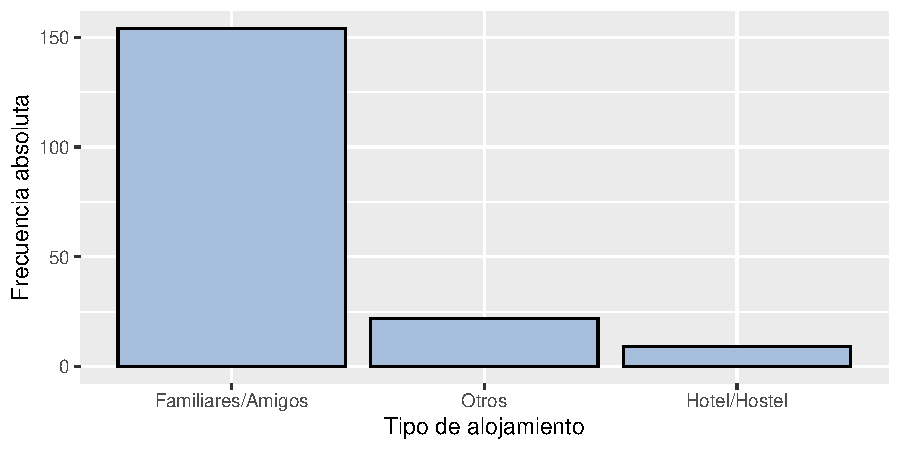
\includegraphics{Informe-Proyectofinal_files/figure-latex/gasto_nulo_alojamiento-1} 

}

\caption{Cantidad de personas que reportan un gasto total nulo, desagregado por el tipo de alojamiento utilizado. En su mayoría, se trata de personas que se hospedan con familiares o amigos}\label{fig:gasto_nulo_alojamiento}
\end{figure}

\begin{figure}[H]

{\centering 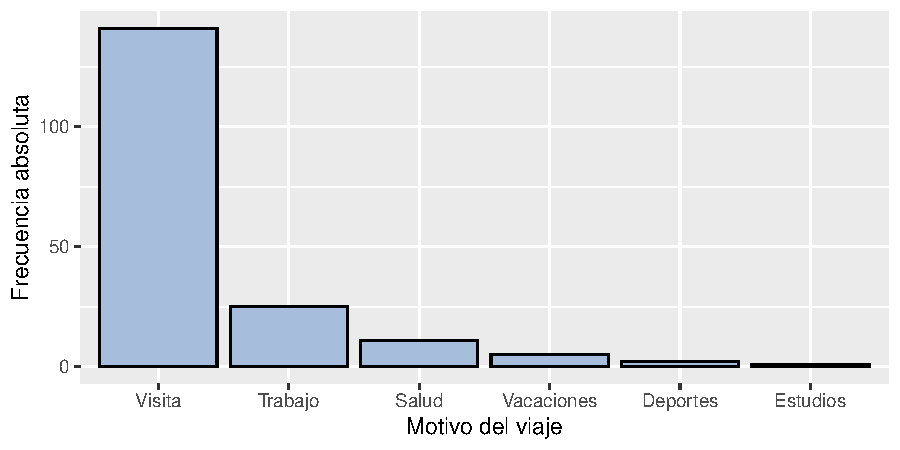
\includegraphics{Informe-Proyectofinal_files/figure-latex/gasto_nulo_motivo-1} 

}

\caption{Cantidad de personas que reportan un gasto total nulo, desagregado por el motivo del viaje. Suele tratarse de individuos que van a visitar familiares y amigos.}\label{fig:gasto_nulo_motivo}
\end{figure}

Por otra parte, se analizó si existían observaciones atípicas, en
términos del gasto total, que pudieran dificultar el análisis. Como
primer paso, se construyó un gráfico de caja y un histograma con la
distribución del gasto (ver figura \ref{fig:boxplot_gasto}).

\begin{figure}[H]

{\centering 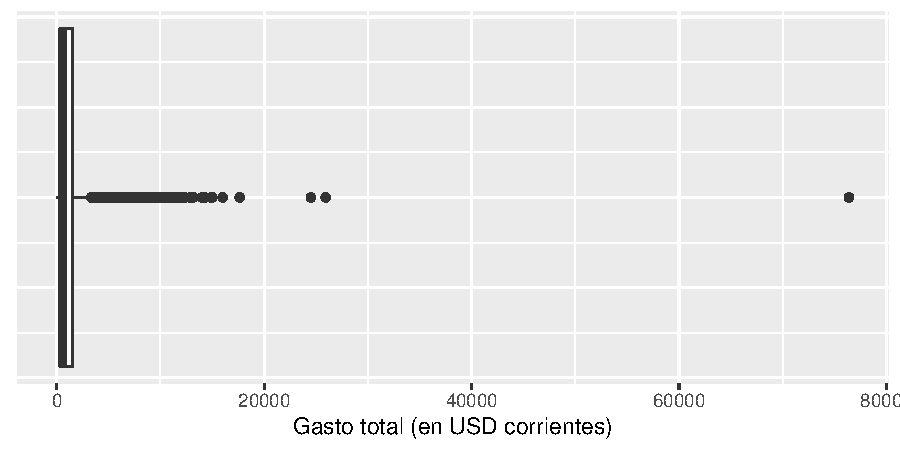
\includegraphics{Informe-Proyectofinal_files/figure-latex/boxplot_gasto-1} 

}

\caption{Gráfico de caja para el gasto total, medido en dólares americanos corrientes. Se aprecian varios valores atípicamente altos.}\label{fig:boxplot_gasto}
\end{figure}

Si bien se advierte que existen múltiples valores extremos, claramente
hay uno que se aleja muchísimo del resto y que alcanza un gasto total de
prácticamente USD 80.000. Dicha observación corresponde a un viaje de 22
días a Europa realizado por un grupo de cuatro personas. Esto equivale a
un gasto medio diario per cápita de casi USD 870, extremadamente alto.
Por lo tanto, se consideró que efectivamente se trata de un
\emph{outlier} y se decidió quitarlo de la base.

A pesar de esta intevención, como muestra la figura
\ref{fig:sin_outliers}, continúa habiendo varios \emph{outliers} en la
distribución del gasto. Esto determina que el correspondiente diagrama
de caja e histograma exhiban una fuerte asimetría hacia la izquierda.
Sin embargo, en este caso, se optó por no removerlas. De lo contrario,
podría distorsionarse el análisis y arribarse a resultados incorrectos.

\begin{figure}[H]

{\centering 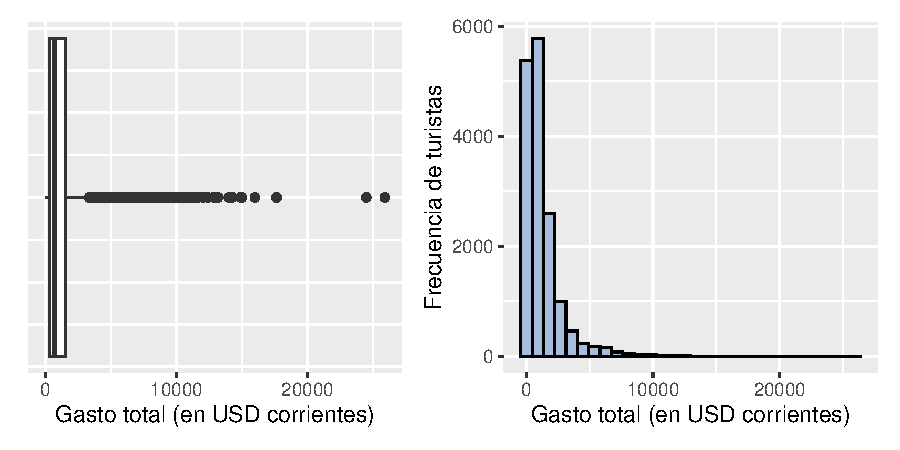
\includegraphics{Informe-Proyectofinal_files/figure-latex/sin_outliers-1} 

}

\caption{Gráfico de caja e histograma para el gasto total en dólares americanos corrientes, sin el valor atípico más extremo.}\label{fig:sin_outliers}
\end{figure}

\hypertarget{cuxe1lculo-del-gasto-medio-diario-por-persona}{%
\subsection{\texorpdfstring{Cálculo del gasto medio diario por persona
\label{calculo_gasto}}{Cálculo del gasto medio diario por persona }}\label{cuxe1lculo-del-gasto-medio-diario-por-persona}}

Antes de explorar los datos para dar respuesta a las interrogantes
planteadas en la sección \ref{problema}, fue necesario analizar las
características de la variable asociada al gasto total. En los metadatos
de la base, no se aclara si esta variable corresponde al gasto por
persona o para todo el grupo. Para responder a esta pregunta, se
construyeron los diagramas de caja de las figuras
\ref{fig:gasto_personas} y \ref{fig:gasto_estadia}.

En la figura \ref{fig:gasto_personas}, se presenta la distribución del
gasto total, desagregada por la cantidad de personas que viajaron con el
encuestado. Para ello, se agrupó las observaciones en cinco categorías.
Se observa que, a medida que aumenta la cantidad de personas en el
grupo, también el gasto total tiende a crecer. Por lo tanto, es
razonable suponer que esta variable efectivamente mide el gasto de todo
el grupo y no sólo del encuestado.

\begin{figure}[H]

{\centering 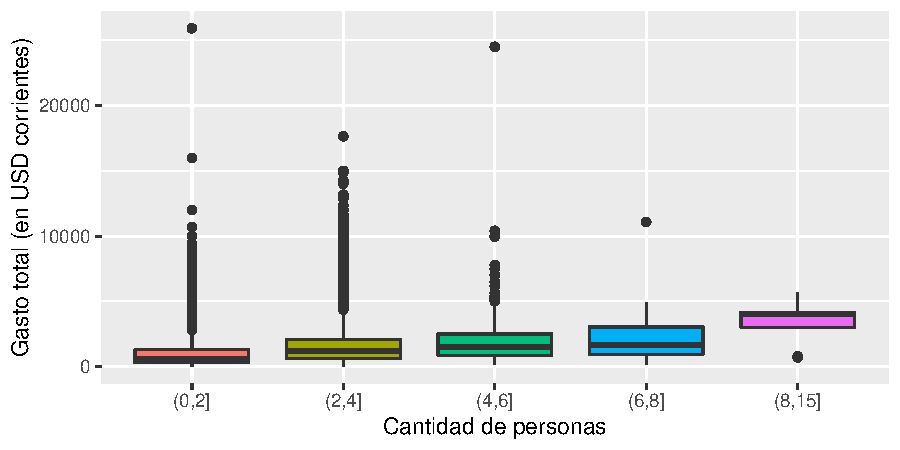
\includegraphics{Informe-Proyectofinal_files/figure-latex/gasto_personas-1} 

}

\caption{Distribución del gasto total en dólares americanos corrientes en función de la catidad de personas que acompañan al encuestado.}\label{fig:gasto_personas}
\end{figure}

Por su parte, para construir el gráfico de la figura
\ref{fig:gasto_estadia}, se discretizó la variable con la cantidad de
días que duró el viaje en función de sus cuartiles. Nuevamente, un
incremento en la cantidad de días se asocia positivamente con el gasto
total del viaje. Por lo tanto, también en este caso puede deducirse que
se trata de un total para todo el viaje y no por día o alguna otra
unidad de medida.

\begin{figure}[H]

{\centering 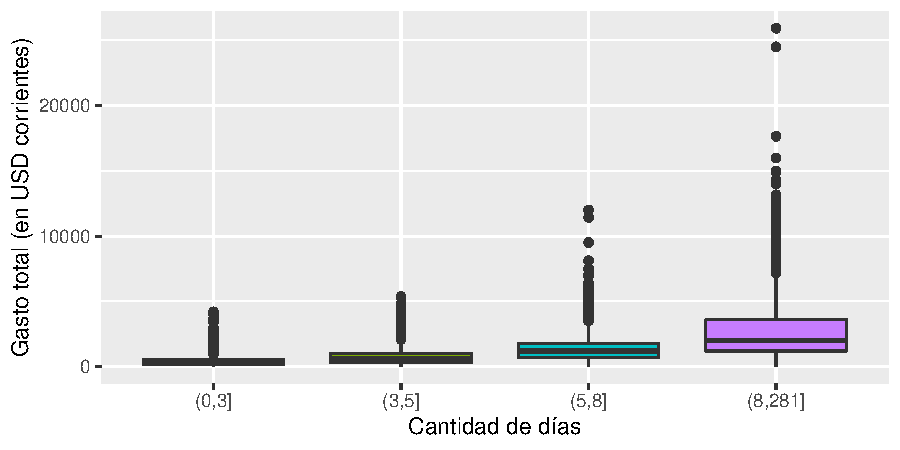
\includegraphics{Informe-Proyectofinal_files/figure-latex/gasto_estadia-1} 

}

\caption{Distribución del gasto total en dólares americanos corrientes en función de la catidad de días de viaje.}\label{fig:gasto_estadia}
\end{figure}

Por lo tanto, para obtener resultados comparables entre encuestados, se
creó una variable que midiera el gasto promedio diario por persona
registrado en cada observación.

\hypertarget{anuxe1lisis-exploratorio}{%
\section{\texorpdfstring{Análisis exploratorio
\label{exploracion}}{Análisis exploratorio }}\label{anuxe1lisis-exploratorio}}

A continuación, se presentan los resultados del análisis exploratorio
realizado con el objetivo de dar respuesta al problema de estudio
planteado en la sección \ref{problema}.

\hypertarget{evoluciuxf3n-de-la-cantidad-de-encuestados}{%
\subsection{Evolución de la cantidad de
encuestados}\label{evoluciuxf3n-de-la-cantidad-de-encuestados}}

En primer lugar, se analizó la evolución mensual en la cantidad de
encuestados entre enero de 2017 y marzo de 2020, antes del inicio de la
pandemia. Como muestra la figura \ref{fig:evolucion}, se observa una
variabilidad mes a mes bastante grande. Probablemente, esto se deba a
que la serie presenta una estacionalidad que hace que, en ciertos meses
del año, haya más salidas de turistas. Este aspecto es tratado más
adelante.

De todos modos, se aprecia que en 2017 se alcanzaron los valores máximos
del turismo. Posteriormente, se observa una caída muy pronunciada entre
el final de 2017 y el inicio del 2018. A su vez, la serie se mantiene
estancada durante todo 2018 y crece durante la mayor parte del 2019.
Finalmente, a partir de los últimos meses de 2019, se advierte un rápido
decrecimiento. Si bien la emergencia sanitaria no queda comprendida en
el los datos analizados, durante este período ya varios países del mundo
registraban altos niveles de contagio de Covid-19.

\begin{figure}[H]

{\centering 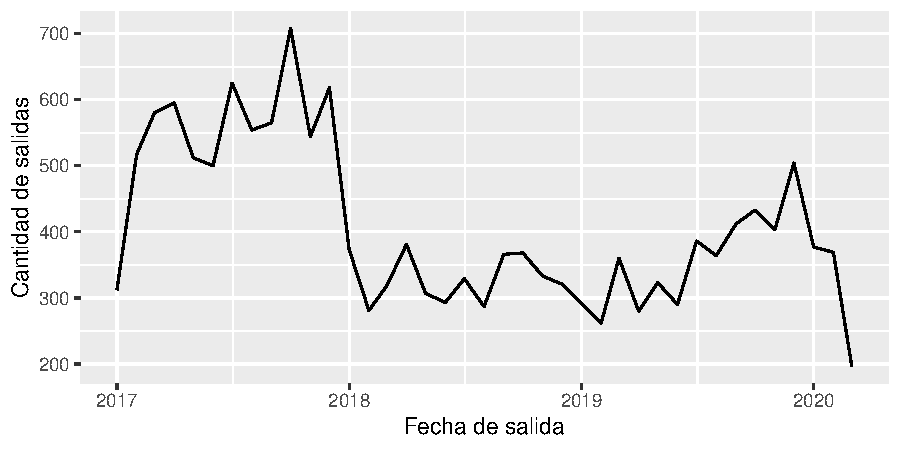
\includegraphics{Informe-Proyectofinal_files/figure-latex/evolucion-1} 

}

\caption{Evolución de la cantidad de encuestados entre enero de 2017 y marzo de 2020.}\label{fig:evolucion}
\end{figure}

\hypertarget{evoluciuxf3n-del-gasto-corriente}{%
\subsection{Evolución del gasto
corriente}\label{evoluciuxf3n-del-gasto-corriente}}

En segundo lugar, se analizó la evolución del gasto medio por día y por
persona entre enero de 2017 y marzo de 2020, expresado en dólarees
corrientes y desagregado por concepto. Para cada mes, se consideró el
promedio en dicha variable para todos los encuestados. Como muestra la
figura \ref{fig:evolucion_gasto}, los mayores gastos corresponden al
transporte internacional. Esto es razonable, en la medida que incluye
pasajes de avión y otros medios de transporte relativamente costosos.
Por su parte, también es considerable la proproción del gasto destinada
a cubrir el alojamiento y la alimentación.

A su vez, es interesante destacar que el gasto en compras es el rubro
que presenta mayor volatilidad. Para algunos meses, llegó a constituir
uno de los componentes más importantes (por ejemplo, a mediados de
2018).

El gasto en transporte local y vinculado a actividades culturales
presenta una estabilidad mucho mayor. Aunque el gasto en transporte
local exhibe un leve aumento durante el período analizado, se mantuvo
cercano a los USD 10 corrientes. Por su parte, el gasto en actividades
culturales oscila en torno a los USD 5.

Finalmente, se observa que el gasto en tours se mantiene cercano a cero
durante todo el período.

\begin{figure}[H]

{\centering 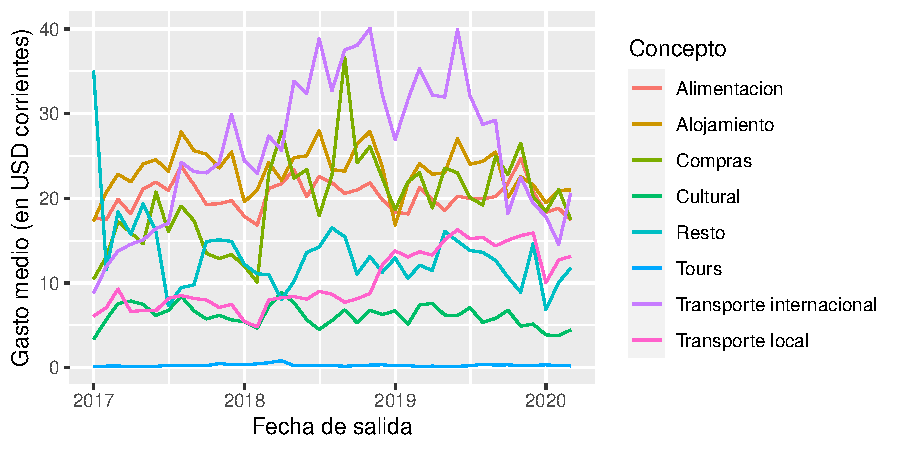
\includegraphics{Informe-Proyectofinal_files/figure-latex/evolucion_gasto-1} 

}

\caption{Evolución del gasto medio diario por persona entre enero de 2017 y marzo de 2020, desagregado por concepto.}\label{fig:evolucion_gasto}
\end{figure}

\hypertarget{evoluciuxf3n-de-la-tendencia-del-gasto-corriente}{%
\subsection{Evolución de la tendencia del gasto
corriente}\label{evoluciuxf3n-de-la-tendencia-del-gasto-corriente}}

Como se analizó en la sección anterior, el gasto medio por día y por
persona presenta variaciones mes a mes bastante grandes. Esto dificulta
visualizar la trayectoria de cada serie en la medida que no resulta
claro el impacto del efecto estacional sobre cada observación.

Para subsanar este problema, se extrajo la tendencia de cada componente
del gasto mediante el método de descomposición de Loess (STL, por su
sigla en inglés). En la figura \ref{fig:evolucion_desest}, se presentan
los resultados.

Se aprecia que la media de los gastos por alojamiento, alimentación,
culturales y en tours es aproximadamente constante a lo largo del
período. Por su parte, las tendencias del gasto en compras y en
transporte local registran un aumento alrededor de 2018.

Sin embargo, lo más llamativo del gráfico es la trayectoria del gasto en
transporte internacional. De esta forma, esta serie crece hasta alcanzar
un máximo a principios de 2019 y luego cae durante el resto del período.
Dado que esta disminución comenzó antes de la pandemia, debe tener su
origen en otras causas (al menos inicialmente).

\begin{figure}[H]

{\centering 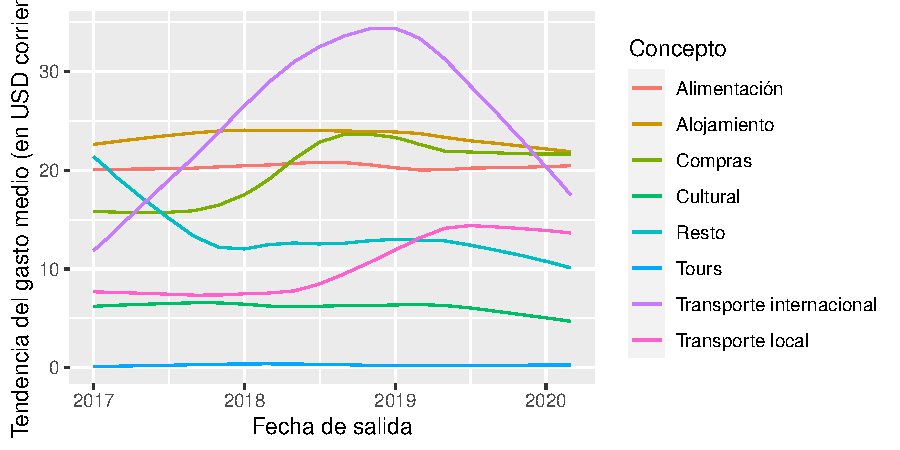
\includegraphics{Informe-Proyectofinal_files/figure-latex/evolucion_desest-1} 

}

\caption{Evolución de la tendencia del gasto medio diario por persona entre enero de 2017 y marzo de 2020, desagregado por concepto.}\label{fig:evolucion_desest}
\end{figure}

Es interesante notar que el comienzo de la reducción en el gasto en
transporte internacional coincide, a grandes rasgos, con el incremento
en el transporte local y en compras. Se plantea la hipótesis de que haya
existido un aumento en los viajes de compras a destinos cercanos como
Argentina. Para indagar en esto, en la figura \ref{fig:lineas_destino}
se presenta la evolución en la cantidad de encuestados por destino del
viaje.

Como muestra el gráfico, a lo largo de todo el período, la mayor parte
de los encuestados viajó a Argentina. Es razonable, entonces, que el
gráfico correspondiente a este país en la figura
\ref{fig:lineas_destino} exhiba una trayectoria muy similar a la de la
figura \ref{fig:evolucion}. En ambos casos, se aprecia una reducción
considerable durante el 2018, seguida por una recuperación durante el
2019 y una nueva caída a principios de 2020. Así, es posible que la
reducción en el gasto en transporte internacional se haya debido a que
los viajes a Argentina son en promedio, más baratos que para otros
destinos.

\begin{figure}[H]

{\centering 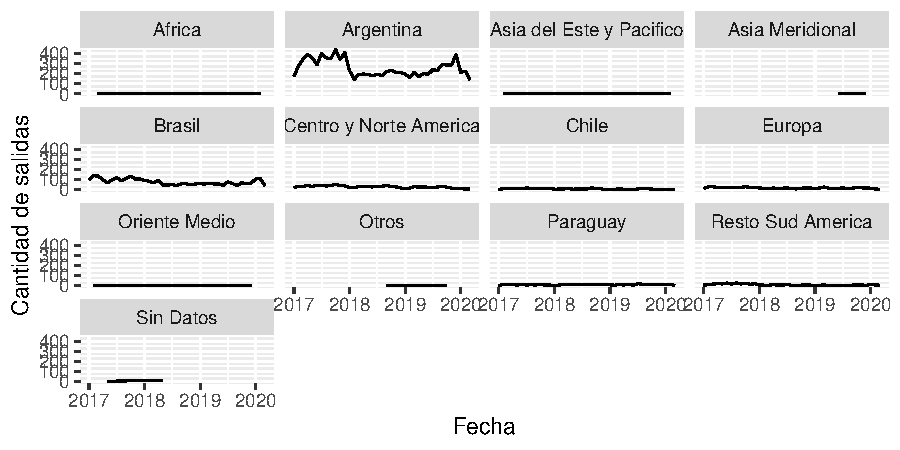
\includegraphics{Informe-Proyectofinal_files/figure-latex/lineas_destino-1} 

}

\caption{Evolución entre enero de 2017 y marzo de 2020 de la cantidad de encuestados por país o región de destino.}\label{fig:lineas_destino}
\end{figure}

\hypertarget{evoluciuxf3n-del-gasto-constante}{%
\subsection{Evolución del gasto
constante}\label{evoluciuxf3n-del-gasto-constante}}

Dado que los datos analizados fueron relevados a lo largo de más de dos
años, es interesante estudiar la evolución del gasto en términos reales.
Esto permite descontar el efecto de la inflación estadounidense y
reflejar mejor la evolución en las decisiones de gasto en dólares de los
encuestados.

En la figura \ref{fig:evolucion_constante}, se presenta la evolución en
el gasto por rubro, deflactado por el IPC de Estados Unidos. Dado que la
inflación en dicho país entre 2017 y 2020 fue baja (alrededor de
\(2\%\)) anual, los resultados no cambian demasiado. De esta manera, más
allá de un cambio de escala, las trayectorias de las series resultan ser
muy similares.

\begin{figure}[H]

{\centering 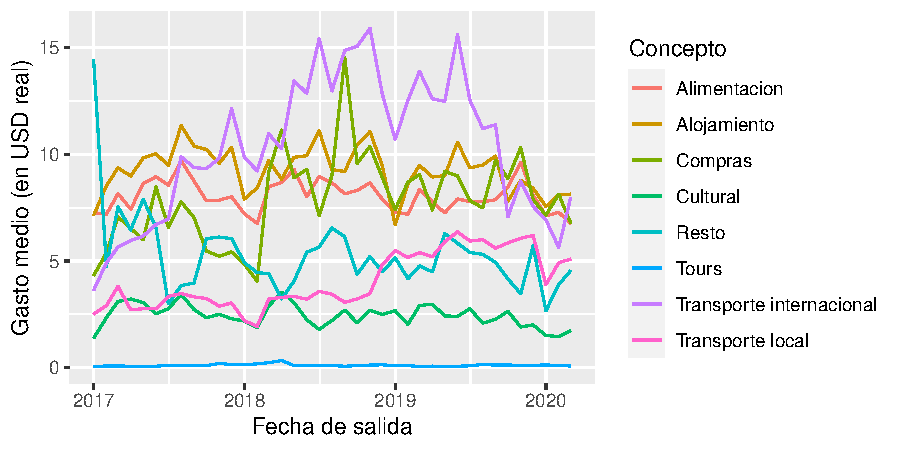
\includegraphics{Informe-Proyectofinal_files/figure-latex/evolucion_constante-1} 

}

\caption{Evolución del gasto medio diario por persona entre enero de 2017 y marzo de 2020, en dólares constantes.}\label{fig:evolucion_constante}
\end{figure}

\hypertarget{distribuciuxf3n-del-gasto-por-destino}{%
\subsection{Distribución del gasto por
destino}\label{distribuciuxf3n-del-gasto-por-destino}}

En lo que resta de la sección \ref{exploracion}, se estudia la
distribución del gasto en función de distintas variables categóricas.
Para facilitar la visualización, se eliminó un dato excepcionalmente
alto, de más de USD 4000 por día per cápita.

En primer lugar, se considera el gasto medio diario por persona por país
o región de destino. En la figura \ref{fig:boxplot1}, se presentan los
correspondientes diagramas de caja.

Los cuartiles más grandes en la distribución del gasto corresponden a
Asia. Además, esta región es la que presenta una mayor dispersión de sus
datos, lo cual determina que su rango intercuartílico sea el más grande.

Los viajes a América del Norte y Central, América del Sur y Europa
registran varios valores inusualmente altos. Así, se observa una
asimetría a la izquierda, con un gran porcentaje del gasto concentrado
en valores ``bajos'' del recorrido.

Sin tomar en cuenta los \emph{outliers}, los viajes a Sudamérica
resultan ser los menos costosos por persona y por día. Luego, le sigue
África, América Central y del Norte, y Europa.

\begin{figure}[H]

{\centering 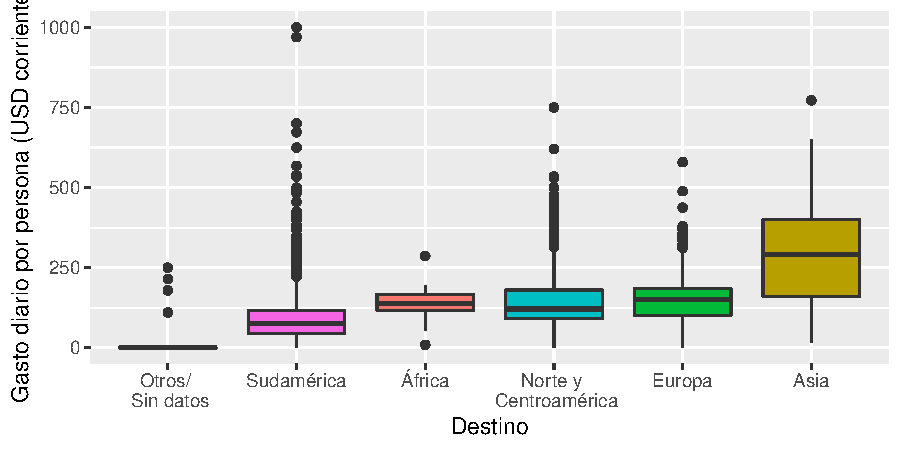
\includegraphics{Informe-Proyectofinal_files/figure-latex/boxplot1-1} 

}

\caption{Diagrama de caja para el gasto medio diario por persona (en dólares corrientes), según país o región de destino.}\label{fig:boxplot1}
\end{figure}

\hypertarget{distribuciuxf3n-del-gasto-por-nivel-educativo}{%
\subsection{Distribución del gasto por nivel
educativo}\label{distribuciuxf3n-del-gasto-por-nivel-educativo}}

En segundo lugar, se analizó la distribución del gasto por máximo nivel
educativo del encuestado (ver figura \ref{fig:boxplot2}). Si se dejan de
lado las observaciones sin datos, se observa que, a mayor nivel
educativo, mayor tiende a ser el gasto medio diario por persona. A
excepción las personas que no tienen primaria completa, todas las
categorías exhiben valores inusuamente grandes. Nuevamente, esto
determina que las distribuciones presenten una fuerte asimetría hacia la
izquierda.

\begin{figure}[H]

{\centering 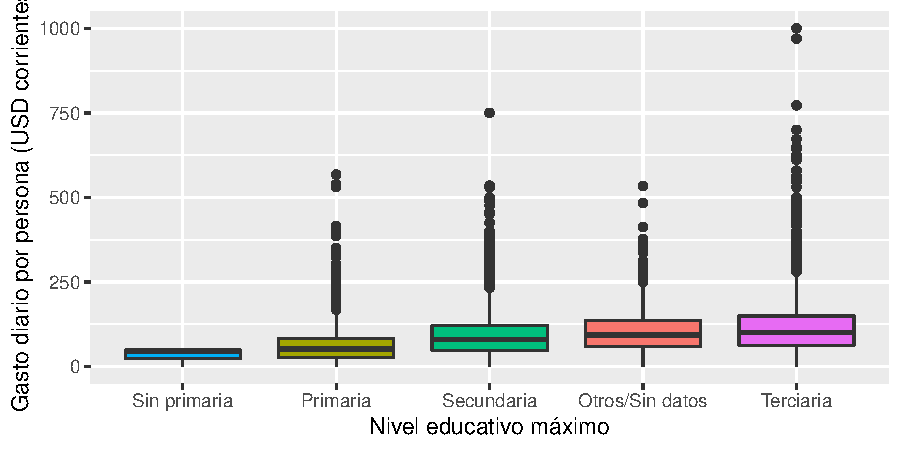
\includegraphics{Informe-Proyectofinal_files/figure-latex/boxplot2-1} 

}

\caption{Diagrama de caja del gasto diario por persona según el máximo nivel educativo alcanzado por el encuestado.}\label{fig:boxplot2}
\end{figure}

\hypertarget{distribuciuxf3n-del-gasto-por-ocupaciuxf3n}{%
\subsection{Distribución del gasto por
ocupación}\label{distribuciuxf3n-del-gasto-por-ocupaciuxf3n}}

El análisis del gasto por ocupación se muestra en la figura
\ref{fig:boxplot3}. Sin tener en cuenta a los individuos para los cuales
no se tiene información, se observa que los menores niveles de gasto
corresponden a los desocupados, seguidos por los inactivos. Los ocupados
presentan los mayores niveles de gasto en términos generales. Además, en
esta categoría se concentra la mayor parte de los \emph{outliers}.

En términos generales, los individuos empleados tienden a percibir
mayores ingresos que los desocupados y los inactivos (entre los que se
encuentran los jubilados), parece razonable que el gasto sea mayor para
esta categoría.

\begin{figure}[H]

{\centering 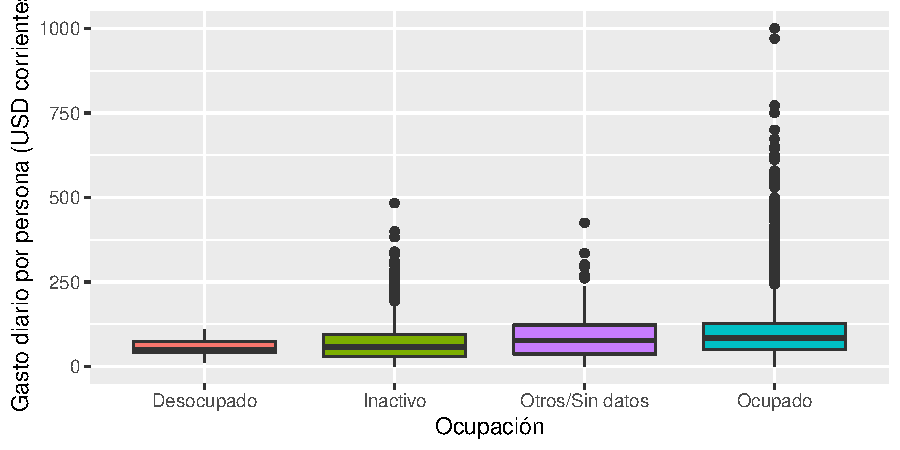
\includegraphics{Informe-Proyectofinal_files/figure-latex/boxplot3-1} 

}

\caption{Diagrama de caja del gasto diario por persona según la ocupación del encuestado.}\label{fig:boxplot3}
\end{figure}

\hypertarget{distribuciuxf3n-del-gasto-por-motivo-del-viaje}{%
\subsection{Distribución del gasto por motivo del
viaje}\label{distribuciuxf3n-del-gasto-por-motivo-del-viaje}}

En la figura \ref{fig:boxplot4}, se presenta la distribución del gasto
por motivo del viaje. Los mayores gastos se dan entre quienes realizan
viajes de compras, lo cual es esperable.

Por el contrario, las personas que viajan para visitar familiares y/o
amigos son las que registran menores niveles de gasto. Como se analizó a
través de las figuras \ref{fig:gasto_nulo_alojamiento} y
\ref{fig:gasto_nulo_motivo}, en ocasiones estas personas reportan gastos
nulos debido a que se hospedan con las personas a las que fueron a ver.

Algo similar ocurre con las personas que viajan por motivos deportivos.
En este caso, suele tratarse de individuos que van a participar de
partidos, competencias, etc., por lo que sus gastos suelen estar
cubiertos por un tercero. Por lo tanto, sus gastos tienden a ser
relativamente bajos.

Es llamativo el hecho de que, luego de quienes viajan de compras, los
individuos que viajan por razones laborales sean los que exhiben mayores
niveles de gasto. \emph{A priori}, no es claro a qué podría deberse
esto.

\begin{figure}[H]

{\centering 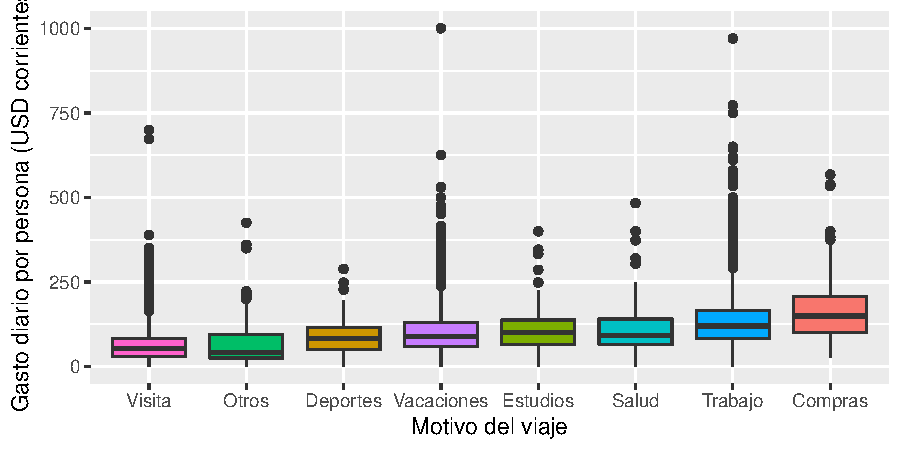
\includegraphics{Informe-Proyectofinal_files/figure-latex/boxplot4-1} 

}

\caption{Diagrama de caja del gasto diario por persona según el motivo del viaje.}\label{fig:boxplot4}
\end{figure}

\hypertarget{distribuciuxf3n-del-gasto-por-tipo-de-alojamiento}{%
\subsection{Distribución del gasto por tipo de
alojamiento}\label{distribuciuxf3n-del-gasto-por-tipo-de-alojamiento}}

Finalmente, se exploró la relación existente entre el tipo de
alojamiento utilizado durante el viaje y el gasto medio diario por
persona. Los resultados se presentan en la figura \ref{fig:boxplot5}.
Los menores niveles de gasto corresponden a quienes se quedan en
campings. Como fue dicho, también quienes se alojan con familiares y
amigos registran un bajo gasto.

Por otra parte, las personas que alquilan un apartamento o cabaña
tienden a gastar menos que los que se quedan en un hotel u hostel. Para
esta última categoría, se advierte una gran dispersión en el gasto, con
una gran cantidad de \emph{outliers}. Probablemente, esto se deba a la
gran variedad de precios de hoteles.

En el extremo superior, la distribución del gasto de quienes se hospedan
en yates o cruceros se concentra en niveles altos del recorrido, lo cual
parece razonable ya que se trata de un tipo de alojamiento ``lujoso''.

\begin{figure}[H]

{\centering 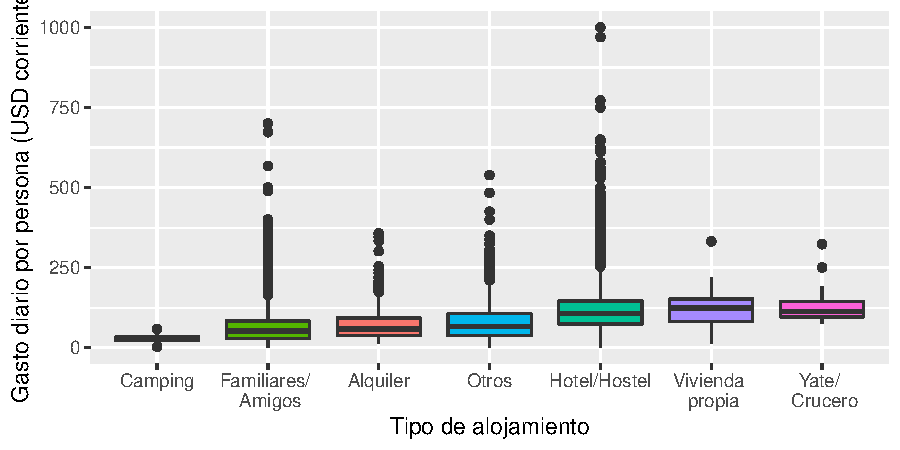
\includegraphics{Informe-Proyectofinal_files/figure-latex/boxplot5-1} 

}

\caption{Diagrama de caja del gasto diario por persona según el tipo de alojamiento.}\label{fig:boxplot5}
\end{figure}

\hypertarget{construcciuxf3n-de-una-aplicaciuxf3n-web}{%
\section{\texorpdfstring{Construcción de una aplicación web
\label{shiny}}{Construcción de una aplicación web }}\label{construcciuxf3n-de-una-aplicaciuxf3n-web}}

\url{https://patriciamartell.shinyapps.io/ShinyApp/}

La aplicación Shiny permite realizar un análisis sobre la base de datos
de turismo emisivo de uruguay detallada en los apartados Introducción y
Problema de estudio y objetivos de este informe. En esta se presentan
visualizaciones relevantes de acuerdo a las variables que se desean
explorar.

La información se organiza en tres pestañas: Componentes del turismo (en
la cual se despliguega un panel de selección de dos hojas: Evolución de
la cantidad de salidas y Evolución del gasto en salidas),
Características del turismo y Serie de tiempo. En la siguiente imagen se
visualiza la pantalla inicial al ingresar a la aplicación de shiny y la
organización de pestañas descrita. Además, en cada una de las pestañas
de la aplicación se dispondrá de un panel de selección de filtro de las
visualizaciones.

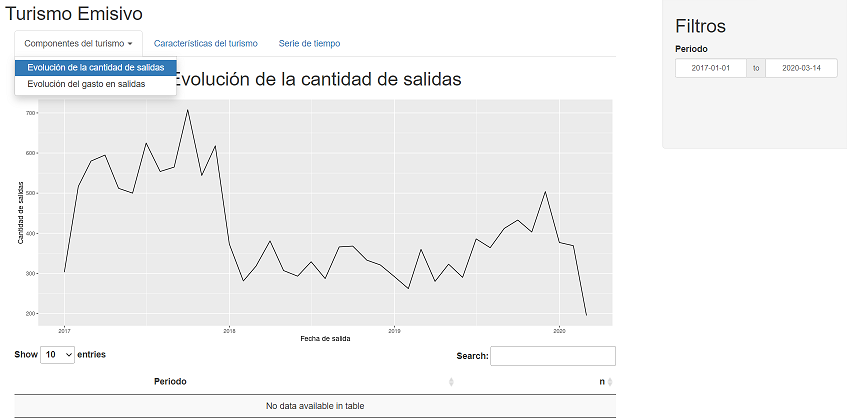
\includegraphics{Imagenes-shiny/imagen1.png} En la pestaña Componentes
del turismo y apartado Evolución de la cantidad de salidas se visualiza
un gráfico de lineas de los datos de turismo emisivo a partir de 2017.
Este apartado cuenta con selección de periodo en el panel de selección
filtros y la opción de brushedpoint sobre la gráfica lo que permite
hacer una selección sobre la visualización y que se despliegue la
cantidad de salidas por mes en formato tabla. En la siguiente imagen se
selecciona el periodo enero 2017 a diciembre 2018 en el panel de filtros
y los tres puntos más altos de dicho periodo en la gráfica, lo que
despliega información de periodo y cantidad de salidas en la tabla para
los puntos seleccionados.

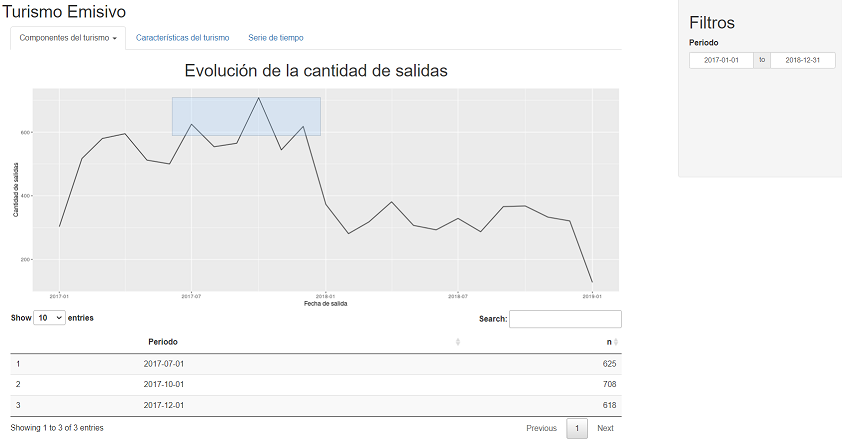
\includegraphics{Imagenes-shiny/imagen2.png} En la pestaña Componentes
del turismo y apartado Evolución del gasto en salidas se visualiza un
gráfico de lineas discriminado por tipo de gasto en turismo emisivo a
partir de 2017. Este apartado cuenta en el panel de selección de filtros
con selección de periodo y selección por Gasto medio o Gasto diario por
persona. Además, esta visualizacíón es Plotly lo que desliega una cajita
de información al pasar sobre cualquier punto de la gráfica como se
visualiza en la siguiente imagen.

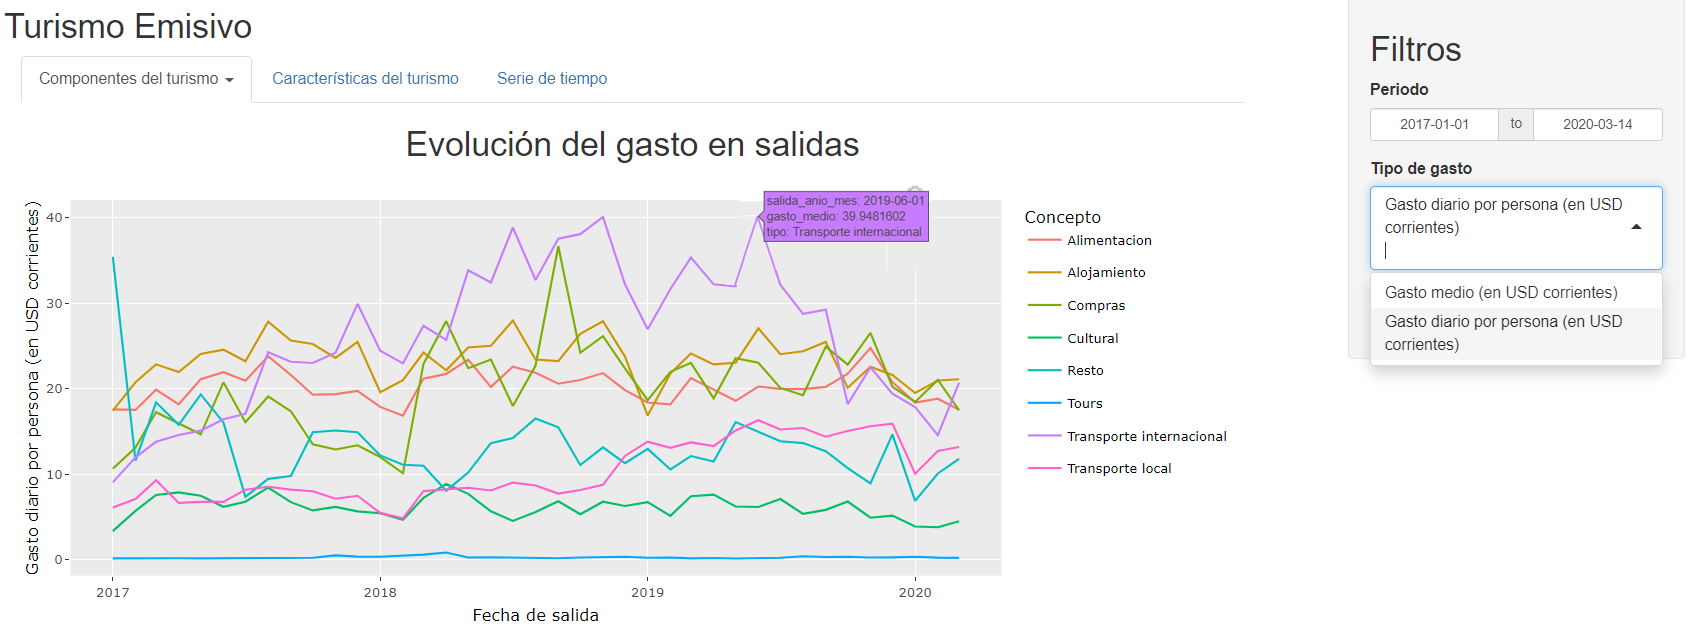
\includegraphics{Imagenes-shiny/imagen3.png}

En la pestaña Características del turismo se visualiza un diagrama de
caja y una tabla con las principales estadísticas de los diagramas de
caja del gasto diario por persona en turismo emisivo a partir de 2017
según una característica de turismo. Esta pestaña cuenta en el panel de
selección de filtros con selección de periodo y selección de
característica de turismo dentro de las cuales se encuentra:
Alojamiento, Destino, Días de estadía, Integrantes por grupo, Motivo,
Nivel educativo máximo y Tipo de ocupación. En otras palabras, se
analiza el gasto diario por persona en base a una de estas variables del
turismo.

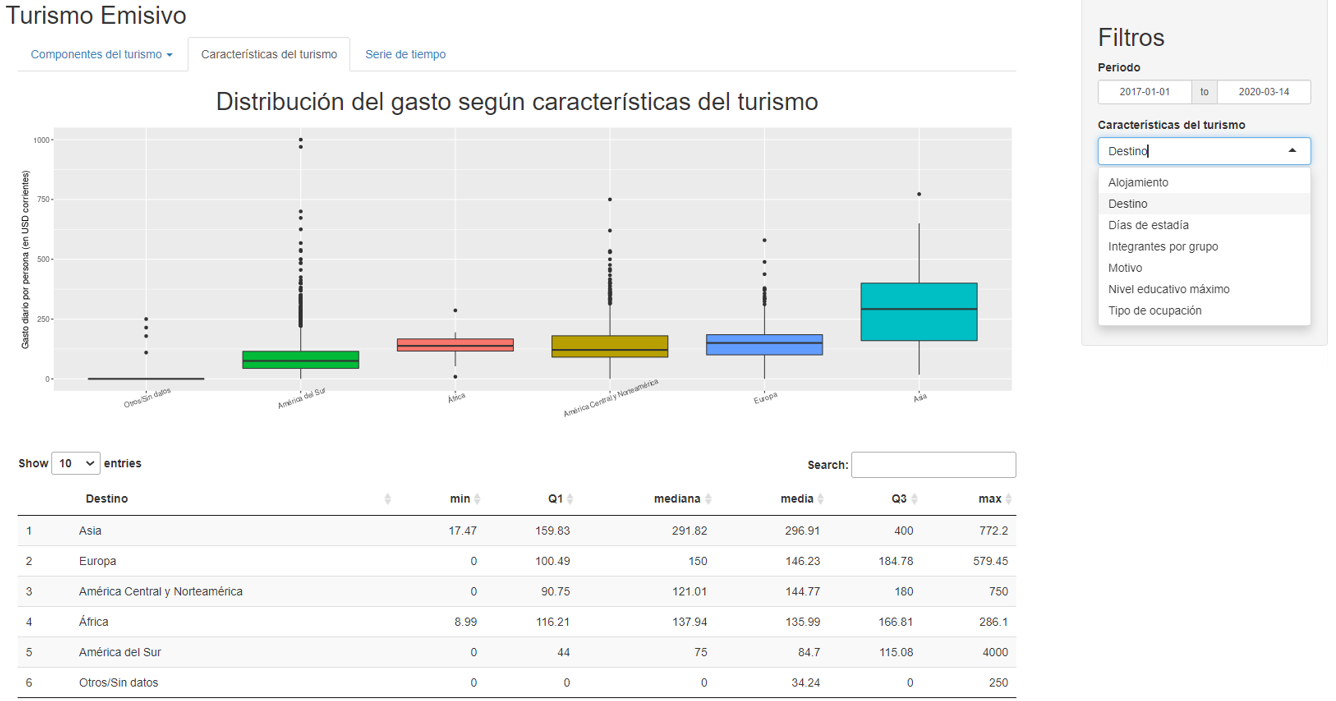
\includegraphics{Imagenes-shiny/imagen4.png}

En la pestaña Serie de tiempo se visualiza la tendencia del gasto medio
desestacionalizado del turismo emisivo a partir de 2017. Esta pestaña
cuenta en el panel de selección de filtros con selección de periodo.
Además, esta visualizacíón es Plotly lo que desliega una cajita de
información al pasar sobre cualquier punto de la gráfica como se
visualiza en la siguiente imagen.

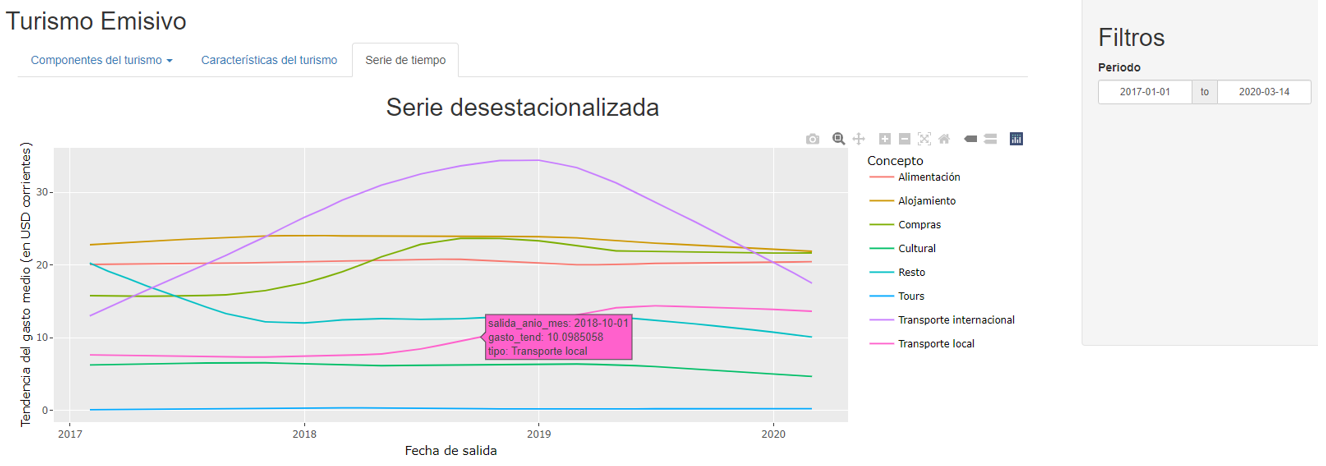
\includegraphics{Imagenes-shiny/imagen5.png}

\hypertarget{conclusiones}{%
\section{\texorpdfstring{Conclusiones
\label{conclusiones}}{Conclusiones }}\label{conclusiones}}

A lo largo de este trabajo, se exploró la última base de datos de
turismo emisivo, publicada por el Ministerio de Turismo. Para un
conjunto de encuestados entre diciembre de 2016 y marzo de 2020, se
relevan datos vinculados al tipo de viaje realizado. Dado que se trató
de una encuesta, para obtener estimaciones insesgadas resulta necesario
expandir la muestra. Sin embargo, en este trabajo se optó por no
utilizarlos. Por lo tanto, los resultados deben ser interpretados con
cautela.

El objetivo principal de este trabajo fue analizar la evolución del
gasto medio diario per cápita de los turistas uruguayos. Para ello, se
consideraron distintos rubros de gastos como transporte, alojamiento y
compras, entre otros. Para ello, se consideró tanto el gasto en términos
corrientes como constantes. Asimismo, se analizó su tendencia de largo
plazo.

A partir de este análisis, se sacaron varias conclusiones interesantes,
entre las que se destaca:

\begin{itemize}
\tightlist
\item
  El transporte internacional constituye el principal componente del
  gasto de los turistas uruguayos en el exterior. En 2017 y 2018, el
  gasto medio mensual por este concepto creció ininterrumpidamente.
  Luego de alcanzar un máximo a principios de 2019, la serie cayó hasta
  marzo de 2020, cuando se decretó la emergencia sanitaria.
\item
  La caída en el transporte internacional coincide con un crecimiento en
  la cantidad de viajes a Argentina. Para este destino, los costos de
  transporte son menores que para otras regiones. Por ende, si bien este
  trabajo no pretende inferir relaciones de causalidad, se plantea la
  hipótesis de que ambos fenómenos estén relacionados.
\item
  Los costos por concepto de alimentación, alojamiento, transporte
  local, actividades culturales tours exhiben una media aproximadamente
  constante a lo largo del tiempo.
\item
  El gasto en compras es, por lejos, el componente más volátil del gasto
  medio diario por persona.
\end{itemize}

Además, se intentó identificar potenciales asociaciones entre el nivel
de gasto y distintas variables categóricas. Los resultados más
relevantes que se hallaron fueron:

\begin{itemize}
\tightlist
\item
  La región de destino más costosa es Asia. Sin embargo, existen varios
  datos inusualmente altos entre quienes viajan a otras partes del
  mundo.
\item
  A mayor nivel educativo del encuestado, mayor tiende a ser el gasto
  total.
\item
  Los individuos ocupados tienden a gastar más que los desempleados y
  los inactivos.
\item
  Quienes viajan para visitar a familiares tienden a gastar menos. Esto
  se debe a que, con frecuencia, se evitan los costos de alojamiento.
\end{itemize}

\renewcommand\refname{Referencias \label{referencias}}
  \bibliography{bibliografia.bib}

\end{document}
